\subsection{Template}
\label{template}

\textbf{Scopo}: Comportamentale \\
\textbf{Raggio d'azione}: Classi

\paragraph{Definizione} Il pattern Template definisce la struttura di un algoritmo all'interno di un metodo, delegando alcuni passi alle sottoclassi (motivo per cui è un pattern class-based). Questo ci sonsente, introducendo sottoclassi diverse, di cambaire il modo in cui i sottopassi vengono eseguiti, lasciando inalterata la struttura dell'algoritmo che è stato inglobato.

\begin{figure}[H]
    \centering
    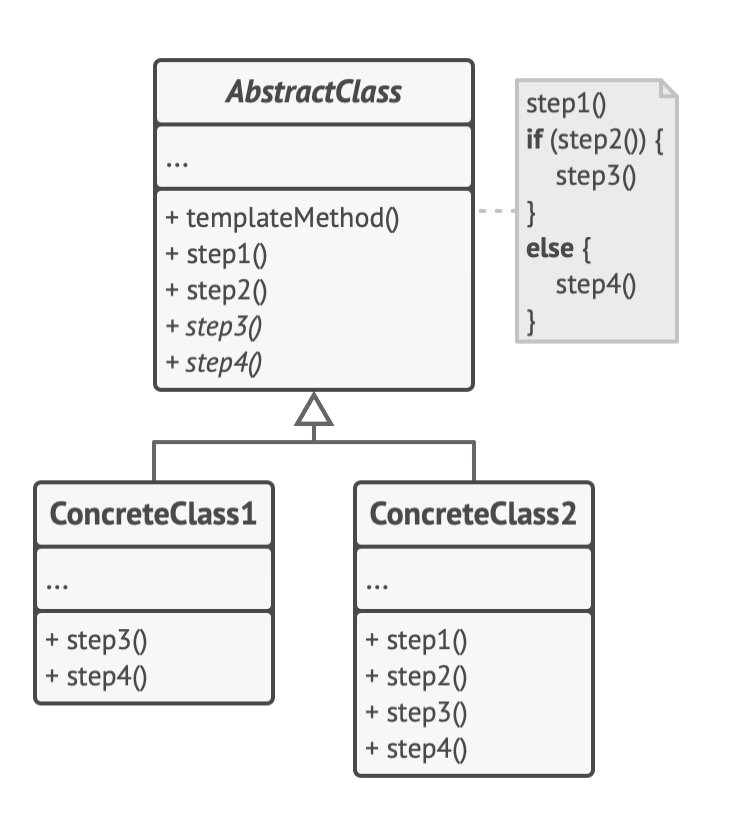
\includegraphics[width=0.5\linewidth]{assets/pattern/template/template-struttura.png}
    \caption{Struttura del pattern}
\end{figure}

\paragraph{Struttura e Conseguenze} Il pattern è composto da:
\begin{itemize}
    \item \textbf{AbstractClass}: dichiara i metodi che agiscono come passaggi di un algoritmo, nonché il metodo \textit{template} vero e proprio che chiama questi metodi in un ordine specifico. I passaggi possono essere dichiarati astratti o avere un'implementazione predefinita.
    \item \textbf{ConcreteClass}: possono sovrascrivere tutti i passaggi, ma non il metodo del modello stesso (template).
\end{itemize}

\begin{figure}[H]
    \centering
    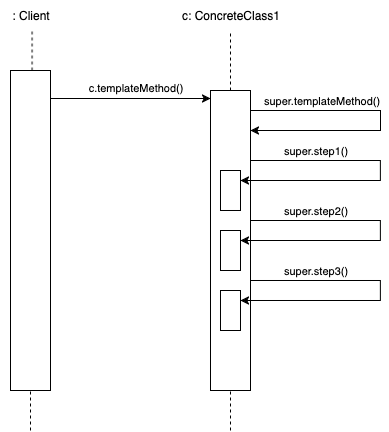
\includegraphics[width=0.5\linewidth]{assets/pattern/template/template-sequence.drawio.png}
\end{figure}

Il pattern permette di rimuovere codice duplicato inserendolo nella AbstractClass, però alcuni client potrebbero essere limitati dallo scheletro fornito di un dato algoritmo. In più i metodi tendono ad essere più difficili da mantenere all'aumentare dei passaggi forniti.



\newpage